\documentclass[a4paper,12pt]{report}
\usepackage{styles/fbe_tez}
\usepackage[utf8]{inputenc} % To use Unicode (e.g. Turkish) characters
\renewcommand{\labelenumi}{(\roman{enumi})}
\usepackage{amsmath, amsthm, amssymb}
 % Some extra symbols
\usepackage{cite}
\usepackage{url}
\usepackage{graphicx}
\usepackage{longtable}
\graphicspath{{figures/}} % Graphics will be here

\usepackage{tikz}
\usetikzlibrary{shapes.geometric, arrows.meta, positioning, fit, calc}

\tikzset{
    block/.style={rectangle, draw, rounded corners=2pt, minimum width=2.4cm, minimum height=0.8cm, align=center, font=\small},
    storage/.style={cylinder, shape border rotate=90, aspect=0.25, draw, minimum height=1.0cm, minimum width=1.6cm, align=center, font=\small},
    actor/.style={circle, draw, minimum size=0.6cm, font=\small},
    arrow/.style={-{Latex[length=2mm]}, thick},
    dashedarrow/.style={-{Latex[length=2mm]}, thick, dashed},
}

\begin{document}

% Title Page
\title{CMPE 492 \\ Digitization of Historical Meteorology Graphs from the Kandilli Observatory Archive}
\author{
Ahmet Sel\c{c}uk Ersoy \\
Kerem Bozkurt \\ \\
Advisor: \\
H. Birkan Y\i{}lmaz
}
\date{}
\maketitle{}
\pagenumbering{roman}
\tableofcontents

\chapter{INTRODUCTION}
\pagenumbering{arabic}

The Kandilli Observatory has been recording atmospheric measurements continuously since the late nineteenth century. The temperature record between 1940 and 1990 survives almost exclusively as paper thermograms~--- continuous ink traces drawn by a mechanical pen on a rotating drum chart. The observatory's archive contains roughly 1,682 high-resolution TIFF scans of these charts, organized by year, chart format, and month, but the actual numerical time series the charts represent has never been captured in machine-readable form. Without that step the data cannot be used in climate reanalysis, statistical studies, or modern visualizations.

The goal of this project is to build a desktop application that turns each scanned thermogram chart into a clean \texttt{(datetime, temperature\,$^\circ$C)} time series ready for downstream analysis. The application is shipped as a single binary, supports macOS and Windows, and is designed to be operated by a researcher with domain knowledge but no programming background. The workflow is human-in-the-loop: an image-processing pipeline produces an initial curve extraction, and a focused editing UI lets the user inspect the overlay, correct individual points, refine specific regions, or redraw a damaged portion of the curve before exporting CSV.

Three properties of the data make automation hard. First, the temperature curve is extremely thin~--- approximately 0.1--0.5\,\% of pixels~--- against a dominant printed grid the curve constantly crosses. Second, the chart was printed on a cylindrical drum, so the vertical grid lines on the scan are not straight but follow a barrel-distorted parabola. Third, the dataset spans five decades and three chart formats (Daily, 4-day, Weekly) with at least nine visually distinct templates that differ in ink color, paper aging, and grid color (orange, green, yellow, pink). A single fixed pipeline cannot handle all of them, so the system was built around per-template color and geometry profiles selected automatically at upload time.

\section{Broad Impact}

The immediate beneficiary is the climate-science community working on the Eastern Mediterranean. A continuous, structured daily temperature record covering the second half of the twentieth century is a building block for trend analysis, validation of reanalysis products, and downscaling of regional climate models. Beyond the specific dataset, the digitization workflow we describe is directly transferable to similar paper archives held by national meteorological services, historical observatories, and citizen-science data-rescue projects. The system replaces a manual transcription task estimated at several minutes per chart with a per-chart workflow of well under a minute for clean scans, with manual editing reserved for the difficult cases. At the dataset scale of 1,682 charts the speed-up is the difference between a feasible undergraduate project and a multi-year manual effort.

A secondary impact is methodological. The choice to use classical computer vision instead of a learned segmentation model was deliberate: training data does not exist, the dataset is too heterogeneous to label exhaustively, and a transparent pipeline can be inspected and corrected by a domain expert. The project demonstrates that careful classical CV plus a well-designed editing UI can meet the accuracy requirements of historical-data rescue without the overhead of model training, GPU infrastructure, or the explainability problems of a neural network.

\section{Ethical Considerations}

The raw chart scans are the property of the Kandilli Observatory and are not redistributed by this project; the application processes images supplied by the user and writes derivative CSV files next to the source image. No identifying or personal information is contained in the data~--- the only signal recorded by the instrument is air temperature~--- so privacy concerns are minimal. The principal ethical risks are scientific rather than personal. An automatically extracted time series carries an implicit claim of accuracy that downstream users may overestimate. We mitigate this in three ways: every extracted point preserves its source pixel coordinates so the original measurement can always be re-derived; the CSV export marks every point that has been manually edited so downstream analyses can filter on provenance; and the application requires explicit per-template calibration by a human before extraction is permitted, so silent miscalibration is unlikely.

\chapter{PROJECT DEFINITION AND PLANNING}
\section{Project Definition}

The project delivers a cross-platform desktop application that takes a scanned thermogram chart (TIFF, PNG, or JPEG) and produces a CSV file of \texttt{(id, time, temperature, x\_pixel, y\_pixel, is\_edited)} records sampled along the temperature curve. The user-facing flow has four stages: (i) upload a scan, automatically classify it into one of nine templates, and reload the last calibration if one exists; (ii) calibrate the grid geometry once per template using a seven-step interactive procedure; (iii) extract the curve in the chosen view, optionally constraining the extraction with starting/ending markers or by drawing a hint stroke; (iv) review, edit, and export. The application bundles a Python sidecar that runs the image-processing pipeline; the Tauri/Rust host process exposes the pipeline through a small set of commands and is responsible for file I/O, temp-file lifecycle, and OS integration.

The deliverable is the application source plus the calibration files for all nine templates we identified in the archive. The project does not ship the original scans, does not perform climatological analysis on the extracted data, and does not provide a cloud or multi-user backend~--- the application runs entirely on the researcher's machine.

\section{Project Planning}
\subsection{Project Time and Resource Estimation}

Active development ran from 4 February 2026 to 4 June 2026, which is roughly eighteen weeks. The two team members worked in parallel, splitting roughly equally between Python image-processing work and TypeScript/Rust application work, with shared time spent on architecture, dataset classification, and weekly advisor meetings. The hardware requirements are modest: a laptop with 8\,GB of RAM and a recent macOS or Windows installation is sufficient. The third-party software dependencies are all open source: Python 3.11+, OpenCV~\cite{bradski2000opencv}, NumPy~\cite{harris2020numpy}, Tauri 2~\cite{tauri}, React~\cite{react}, and Zustand~\cite{zustand}. No paid services, no GPU, and no cloud infrastructure are required.

\subsection{Success Criteria}

We adopted three criteria, in order of importance.

\begin{enumerate}
    \item \textbf{Faithful extraction on a clean scan.} On a representative scan with intact ink and a clearly printed grid, the extracted curve, when overlaid back on the image, must lie on the ink trace at visual inspection across the full time span of the chart. This is the bar that says the pipeline is working at all.
    \item \textbf{Recoverable extraction on a degraded scan.} On a scan with stains, fading, handwritten notations, or partial loss of ink, the application must allow a domain expert to reach the same final accuracy as the clean case within a few minutes of editing~--- through point-level drag, region refinement, or freehand redraw with snap-to-curve.
    \item \textbf{Reproducible export.} Re-extracting the same image with the same calibration must produce the same CSV bit-for-bit, and the CSV must mark every manually edited point so downstream users can filter on provenance.
\end{enumerate}

\subsection{Risk Analysis}

Five risks were identified at the start of the project and tracked throughout. Table~\ref{table:risks} summarizes them along with the mitigation that was adopted.

\begin{table}[thbp]
\vskip\baselineskip
\caption[Project risks and mitigations]{Risk register and adopted mitigations.}
\begin{center}
\begin{tabular}{|p{4.2cm}|c|c|p{6.2cm}|} \hline
\textbf{Risk} & \textbf{Prob.} & \textbf{Impact} & \textbf{Mitigation} \\\hline
Curve too thin to extract reliably & High & High & Per-template color profiles; sliding-window Y tracking with median consensus; MAD outlier removal. \\\hline
Curved grid mis-aligns the time axis & High & High & Cylindrical model $x = \text{linearX} + a\,(y-c_y)^2$ fit during calibration; per-template calibration file. \\\hline
Heterogeneous templates break a single pipeline & High & Medium & Automatic template classification at upload; nine independent color profiles and calibration files. \\\hline
Cross-platform packaging issues & Medium & Medium & Tauri sidecar pattern; tested on macOS first, ported to Windows in last sprint. \\\hline
User error during calibration silently corrupts output & Medium & High & Seven-step guided modal; alignment-only re-entry that reuses existing calibration; CSV marks every edited point. \\\hline
\end{tabular}
\label{table:risks}
\end{center}
\end{table}

\subsection{Team Work}

Both authors were equal contributors and held joint responsibility for all major architectural decisions. The day-to-day split was vertical~--- each person owned a coherent slice of the stack so that pull requests rarely conflicted~--- with shared ownership of integration, testing, and writing. Table~\ref{table:teamwork} summarizes the split.

\begin{table}[thbp]
\vskip\baselineskip
\caption[Team work distribution]{Vertical responsibility split. All architecture and process work was shared.}
\begin{center}
\begin{tabular}{|p{5.5cm}|p{4.5cm}|p{4.5cm}|} \hline
\textbf{Area} & \textbf{Ahmet Sel\c{c}uk Ersoy} & \textbf{Kerem Bozkurt} \\\hline
Desktop host (Tauri/Rust) and IPC layer & Primary & Reviewer \\\hline
React UI, workspace, modals, drag-drop & Primary & Reviewer \\\hline
Zustand stores, edit history, CSV export & Primary & Reviewer \\\hline
Python pipeline core (preprocess, segmenter) & Reviewer & Primary \\\hline
Template detector and per-template profiles & Reviewer & Primary \\\hline
Calibration processor and geometry math & Reviewer & Primary \\\hline
Dataset classification (nine templates) & Joint & Joint \\\hline
Architecture, planning, advisor meetings & Joint & Joint \\\hline
Testing and integration & Joint & Joint \\\hline
Report writing & Joint & Joint \\\hline
\end{tabular}
\label{table:teamwork}
\end{center}
\end{table}

\chapter{RELATED WORK}

The chart-digitization problem has been studied at three levels of generality. At the most general level are open-source tools such as WebPlotDigitizer~\cite{webplotdigitizer} and Engauge Digitizer~\cite{engauge}, which let a user calibrate two axes by clicking and then mark points on a plotted curve. They are excellent for one-off figures but assume a printed chart with a straight grid, a single short curve, and a willing human ready to click every point. They do not scale to a 1,682-image archive.

At the next level are dedicated systems for scientific-document figure mining. These typically combine vector-graphics extraction from PDFs with deep-learning recognition of axes and curves. They target born-digital figures, not scanned analog instrument output, and their assumptions about clean grids and well-defined legends do not transfer.

At the most specific level is the historical-climate data-rescue literature. The IEDRO initiative~\cite{iedro} and the BAMS inventory by Br{\"o}nnimann et al.~\cite{cruz2019atmospheric} catalogue archives in the same condition as Kandilli's: paper records, multiple chart formats, decades of drift. The community has converged on a human-in-the-loop workflow~--- automate where possible, expose the result for review, capture corrections~--- which is exactly the model this project adopts.

On the algorithmic side, the pipeline reuses classical building blocks: CLAHE for contrast normalization~\cite{zuiderveld1994clahe}, bilateral filtering for edge-preserving smoothing~\cite{tomasi1998bilateral}, the Hough line transform for grid detection~\cite{duda1972hough}, and MAD for robust outlier rejection~\cite{leys2013mad}. We considered a learned segmentation model (U-Net~\cite{ronneberger2015unet}) but rejected it: training data did not exist, hand-labeling enough thermograms to cover nine templates plus aging variations was out of scope, and a transparent classical pipeline could be calibrated and audited by the user. The interesting contribution of this project is therefore not algorithmic novelty but the per-template profile system, the cylindrical-grid calibration, and the human-in-the-loop editing UI tying them together.

\chapter{METHODOLOGY}

The pipeline is six logical stages with one classifier at the front (Figure~\ref{fig:pipeline}). Each stage has a single responsibility and writes its output to a typed dataclass that the next stage consumes.

\begin{figure}[h!]
\centering
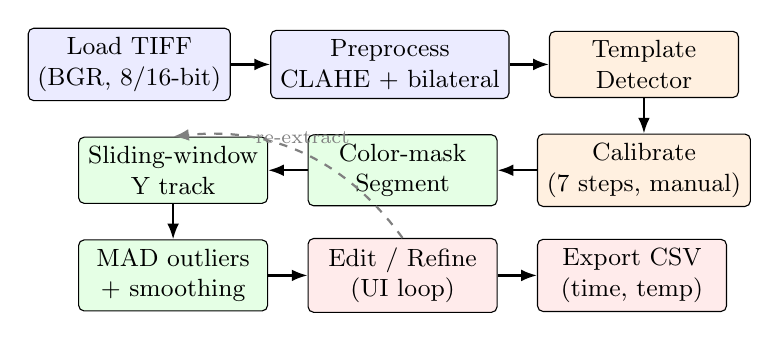
\begin{tikzpicture}[node distance=0.45cm and 0.5cm]
    \node[block, fill=blue!8] (load) {Load TIFF\\(BGR, 8/16-bit)};
    \node[block, right=of load, fill=blue!8] (prep) {Preprocess\\CLAHE + bilateral};
    \node[block, right=of prep, fill=orange!12] (det) {Template\\Detector};
    \node[block, below=of det, fill=orange!12] (cal) {Calibrate\\(7 steps, manual)};
    \node[block, left=of cal, fill=green!10] (seg) {Color-mask\\Segment};
    \node[block, left=of seg, fill=green!10] (track) {Sliding-window\\Y track};
    \node[block, below=of track, fill=green!10] (clean) {MAD outliers\\+ smoothing};
    \node[block, right=of clean, fill=red!8] (edit) {Edit / Refine\\(UI loop)};
    \node[block, right=of edit, fill=red!8] (exp) {Export CSV\\(time, temp)};
    \draw[arrow] (load) -- (prep);
    \draw[arrow] (prep) -- (det);
    \draw[arrow] (det) -- (cal);
    \draw[arrow] (cal) -- (seg);
    \draw[arrow] (seg) -- (track);
    \draw[arrow] (track) -- (clean);
    \draw[arrow] (clean) -- (edit);
    \draw[arrow] (edit) -- (exp);
    \draw[dashedarrow, gray] (edit.north) to[bend right=30] node[above, font=\scriptsize]{re-extract} (track.north);
\end{tikzpicture}
\caption{End-to-end processing pipeline. Blue stages run automatically on upload; orange stages run once per template and are persisted; green stages run on every curve request; red stages are user-driven.}
\label{fig:pipeline}
\end{figure}

\textbf{Preprocessing} normalizes color space and bit depth to BGR 8-bit, applies a bilateral filter ($d=9$, $\sigma_{\text{color}}=\sigma_{\text{space}}=75$) to denoise without destroying the ink edge, and runs CLAHE in LAB color space (clip 2.0, $8{\times}8$ tiles) on the L channel only. The result is then handed to the template detector or, in production, used directly as the input to segmentation.

\textbf{Template detection} converts a $400\times120$ resize of the scan into a 150-feature vector~--- aspect ratio buckets, vertical-line density via Sobel + FFT, left/right/top edge variance and Canny edge density, BGR means in five regions, an 18-bin hue histogram in the chart center, three full BGR 24-bin histograms, and corner statistics. A weighted combination of cosine similarity and normalized Euclidean distance against pre-computed signatures for the nine templates picks the best match. The confidence is the best score scaled by its ratio to the runner-up.

\textbf{Calibration} is interactive and persisted per template. The user performs three horizontal steps (mark top horizontal line, mark its rightmost point for rotation, enter the temperature value and spacing) and four vertical steps (mark a vertical line's top and bottom, enter the reference hour, set the curvature center and slider). The processor stores the rotation angle, horizontal/vertical spacings, line positions, and the curvature coefficient $a$ in the cylindrical model $x = x_{\text{ref}} + a\,(y - c_y)^2$.

\textbf{Curve segmentation} is the core stage. A binary mask of curve pixels is built using RGB rules tuned per template profile (e.g., for the dark-blue-ink-on-orange-grid \texttt{haftalik-2} template, $\text{maxRGB}\le 120$, saturation between 5 and 100, with a grayscale fallback for pencil-like traces). A sliding window centered on an expected $y$ value walks left to right across the columns, taking the median of mask pixels within a $\pm 5$ pixel tight band when possible and a $\pm 300$ pixel coarse band as fallback; a configurable maximum jump $\Delta y_{\max}=20$ pixels per column keeps the tracker from leaping to a stamp or handwriting. The output of this stage is a column-indexed raw $y$ vector.

\textbf{Refinement} interpolates over short gaps, builds a wide-window reference curve (moving median width 151, Gaussian $\sigma=18$, kernel 81), refines each column to lie within $\pm 40$ pixels of the reference, removes outliers using a MAD threshold scaled by 4.0, and smooths the result with a length-3 moving median followed by a length-5 Gaussian. Top- and bottom-clipped columns are snapped to the grid boundary so an out-of-range portion of the curve traces the edge rather than being interpolated diagonally across a gap.

\textbf{Export} converts pixel coordinates to time using the curvature-corrected vertical line model and to temperature by linear interpolation between adjacent horizontal grid lines. The CSV is written next to the source image and contains \texttt{(id, time, temperature, xValue, yValue, isEdited)}~--- the last column is only emitted when at least one point in the curve has been manually edited.

\chapter{REQUIREMENTS SPECIFICATION}

The application supports a single user~--- a researcher working with the Kandilli archive on their own laptop~--- and the use-case set is therefore narrow. Figure~\ref{fig:usecase} summarizes the relationships.

\begin{figure}[h!]
\centering
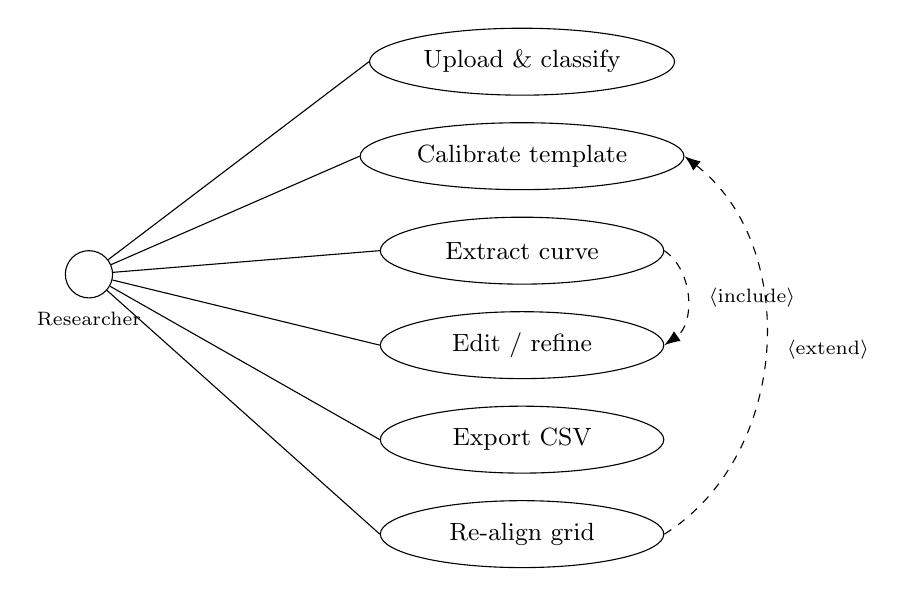
\begin{tikzpicture}[font=\small]
    \node[actor] (user) at (0,0) {};
    \node[below=0.05cm of user, font=\scriptsize] {Researcher};
    \node[draw, ellipse, minimum width=3.6cm, minimum height=0.85cm] (uc1) at (5.5, 2.7)  {Upload \& classify};
    \node[draw, ellipse, minimum width=3.6cm, minimum height=0.85cm] (uc2) at (5.5, 1.5)  {Calibrate template};
    \node[draw, ellipse, minimum width=3.6cm, minimum height=0.85cm] (uc3) at (5.5, 0.3)  {Extract curve};
    \node[draw, ellipse, minimum width=3.6cm, minimum height=0.85cm] (uc4) at (5.5, -0.9) {Edit / refine};
    \node[draw, ellipse, minimum width=3.6cm, minimum height=0.85cm] (uc5) at (5.5, -2.1) {Export CSV};
    \node[draw, ellipse, minimum width=3.6cm, minimum height=0.85cm] (uc6) at (5.5, -3.3) {Re-align grid};
    \draw (user) -- (uc1.west);
    \draw (user) -- (uc2.west);
    \draw (user) -- (uc3.west);
    \draw (user) -- (uc4.west);
    \draw (user) -- (uc5.west);
    \draw (user) -- (uc6.west);
    \draw[-{Latex[length=2mm]}, dashed] (uc3.east) to[bend left=55] node[midway, right=0.15cm, font=\scriptsize]{$\langle$include$\rangle$} (uc4.east);
    \draw[-{Latex[length=2mm]}, dashed] (uc6.east) to[bend right=55] node[midway, right=0.15cm, font=\scriptsize]{$\langle$extend$\rangle$} (uc2.east);
\end{tikzpicture}
\caption{Use-case diagram. A single researcher actor drives all six top-level use cases; editing is included by extraction and re-alignment extends calibration.}
\label{fig:usecase}
\end{figure}

\textbf{Functional requirements.} The application must accept TIFF, PNG, or JPEG input either through a file dialog or drag-and-drop. It must classify the input into one of the nine templates and surface the confidence and all candidate scores so the user can override. It must require an explicit per-template calibration before allowing extraction; the alignment modal must let the user re-align an existing calibration in place without forcing a full recalibration. It must extract the curve automatically when the user switches to curve view, accept optional segment-level starting and ending markers, accept freehand drawing as a hint that is snapped to the curve, and accept a rectangular refine area to re-extract a local region. It must support per-point dragging, multi-point deletion, undo/redo, and a reset-to-raw action. It must export CSV next to the source image and offer Reveal-in-Finder and Open-with-default-app actions on the result.

\textbf{Non-functional requirements.} The desktop binary must run on macOS and Windows. A complete extract on a typical 4\,Mpx scan must finish in under three seconds on a laptop without a discrete GPU. Re-extraction with the same calibration must be bit-for-bit deterministic. All temporary files written for rotation correction must be cleaned up on app exit and on new-image load. The application must function fully offline.

\chapter{DESIGN}

\section{Information Structure}

The application is filesystem-oriented and does not use a relational database. Long-lived state is held in three on-disk artifacts: the source images chosen by the user, one calibration JSON per template under \texttt{backend/calibrations/}, and the CSV exports the application writes next to each source image. Short-lived state (the loaded image, the current extraction, the edit history, the drawing strokes, the refine rectangle) lives in four Zustand stores in the frontend. Figure~\ref{fig:er} shows the entity relationships that exist in the calibration JSON; everything else is per-session.

\begin{figure}[h!]
\centering
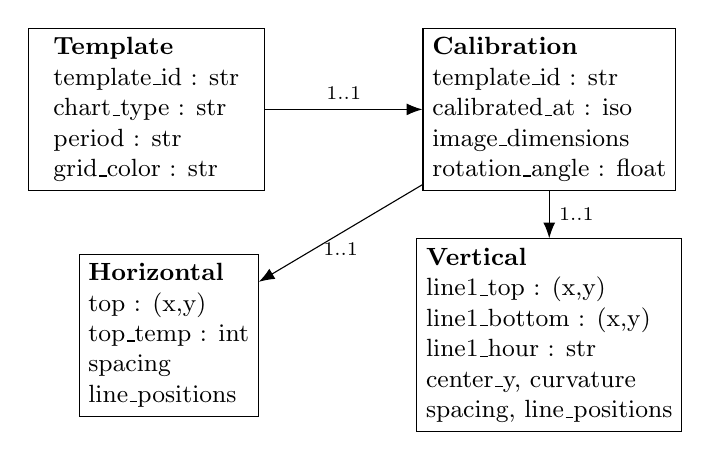
\begin{tikzpicture}[node distance=0.5cm, font=\small]
    \node[draw, rectangle, minimum width=3cm, align=left] (tpl) {\textbf{Template}\\template\_id : str\\chart\_type : str\\period : str\\grid\_color : str};
    \node[draw, rectangle, right=2cm of tpl, align=left] (cal) {\textbf{Calibration}\\template\_id : str\\calibrated\_at : iso\\image\_dimensions\\rotation\_angle : float};
    \node[draw, rectangle, below=0.6cm of cal, align=left] (ver) {\textbf{Vertical}\\line1\_top : (x,y)\\line1\_bottom : (x,y)\\line1\_hour : str\\center\_y, curvature\\spacing, line\_positions};
    \node[draw, rectangle, left=2cm of ver, align=left] (hor) {\textbf{Horizontal}\\top : (x,y)\\top\_temp : int\\spacing\\line\_positions};
    \draw[-{Latex[length=2mm]}] (tpl) -- node[above, font=\scriptsize]{1..1} (cal);
    \draw[-{Latex[length=2mm]}] (cal) -- node[right, font=\scriptsize]{1..1} (ver);
    \draw[-{Latex[length=2mm]}] (cal) -- node[below, font=\scriptsize]{1..1} (hor);
\end{tikzpicture}
\caption{Entity model held in each calibration JSON file. The nine templates each have at most one calibration record.}
\label{fig:er}
\end{figure}

\section{Information Flow}

The interaction between user, frontend, Rust host, and Python sidecar is summarized in Figure~\ref{fig:sequence}. The host is a thin shell: it receives a Tauri command, spawns \texttt{python3 backend/main.py} with the right arguments, and parses the JSON response. All image-processing logic lives in the sidecar.

\begin{figure}[h!]
\centering
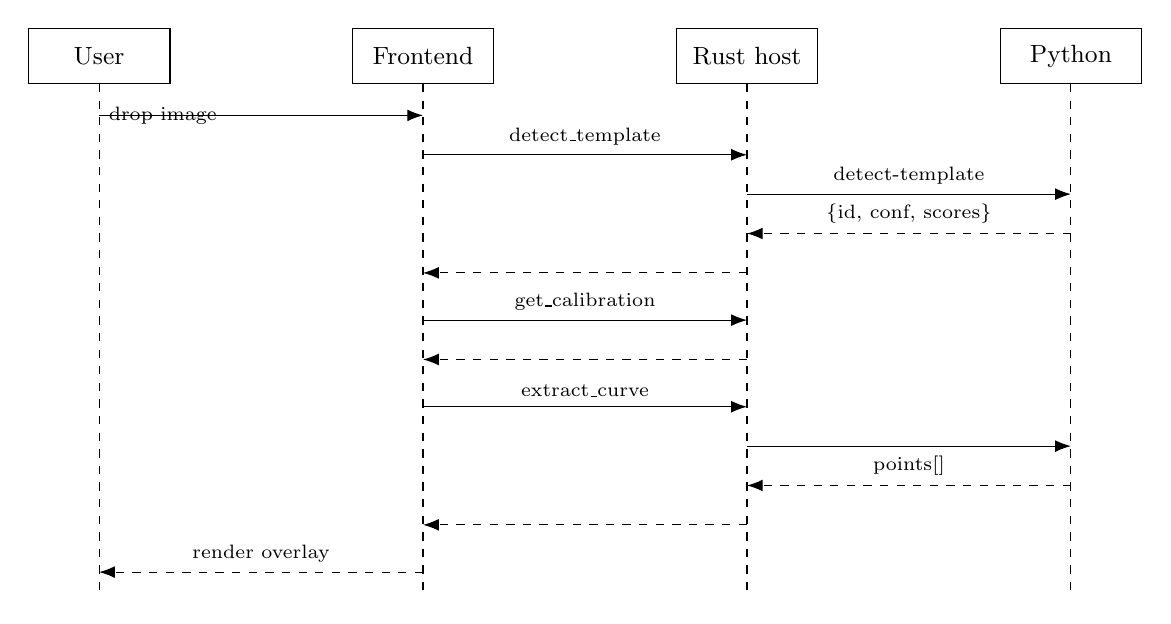
\begin{tikzpicture}[node distance=2.3cm, font=\small]
    \node[draw, rectangle, minimum width=1.8cm, minimum height=0.7cm] (u) {User};
    \node[draw, rectangle, right=of u, minimum width=1.8cm, minimum height=0.7cm] (f) {Frontend};
    \node[draw, rectangle, right=of f, minimum width=1.8cm, minimum height=0.7cm] (r) {Rust host};
    \node[draw, rectangle, right=of r, minimum width=1.8cm, minimum height=0.7cm] (p) {Python};
    \foreach \n in {u,f,r,p} { \draw[dashed] (\n.south) -- ($(\n.south) + (0,-6.5)$); }
    \node[anchor=west, font=\scriptsize] at ($(u.south) + (0,-0.4)$) {drop image};
    \draw[-{Latex[length=2mm]}] ($(u.south) + (0,-0.4)$) -- ($(f.south) + (0,-0.4)$);
    \draw[-{Latex[length=2mm]}] ($(f.south) + (0,-0.9)$) -- node[above, font=\scriptsize]{detect\_template} ($(r.south) + (0,-0.9)$);
    \draw[-{Latex[length=2mm]}] ($(r.south) + (0,-1.4)$) -- node[above, font=\scriptsize]{detect-template} ($(p.south) + (0,-1.4)$);
    \draw[-{Latex[length=2mm]}, dashed] ($(p.south) + (0,-1.9)$) -- node[above, font=\scriptsize]{\{id, conf, scores\}} ($(r.south) + (0,-1.9)$);
    \draw[-{Latex[length=2mm]}, dashed] ($(r.south) + (0,-2.4)$) -- ($(f.south) + (0,-2.4)$);
    \draw[-{Latex[length=2mm]}] ($(f.south) + (0,-3.0)$) -- node[above, font=\scriptsize]{get\_calibration} ($(r.south) + (0,-3.0)$);
    \draw[-{Latex[length=2mm]}, dashed] ($(r.south) + (0,-3.5)$) -- ($(f.south) + (0,-3.5)$);
    \draw[-{Latex[length=2mm]}] ($(f.south) + (0,-4.1)$) -- node[above, font=\scriptsize]{extract\_curve} ($(r.south) + (0,-4.1)$);
    \draw[-{Latex[length=2mm]}] ($(r.south) + (0,-4.6)$) -- ($(p.south) + (0,-4.6)$);
    \draw[-{Latex[length=2mm]}, dashed] ($(p.south) + (0,-5.1)$) -- node[above, font=\scriptsize]{points[]} ($(r.south) + (0,-5.1)$);
    \draw[-{Latex[length=2mm]}, dashed] ($(r.south) + (0,-5.6)$) -- ($(f.south) + (0,-5.6)$);
    \draw[-{Latex[length=2mm]}, dashed] ($(f.south) + (0,-6.2)$) -- node[above, font=\scriptsize]{render overlay} ($(u.south) + (0,-6.2)$);
\end{tikzpicture}
\caption{Sequence of interactions for the upload-to-extract path. Calibration writes follow the same shape; export bypasses Python and serializes CSV directly in the frontend.}
\label{fig:sequence}
\end{figure}

\section{System Design}

The system is partitioned into four cooperating pieces. The React frontend renders the workspace, modals, and overlays. Four Zustand stores hold per-session state: \texttt{imageStore} for the loaded scan and detected template, \texttt{calibrationStore} for the modal flow, \texttt{curveStore} for extracted points, edit history, drawing strokes, refine rectangle, and undo/redo, and \texttt{dataStore} for export metadata. The Rust host exposes eleven Tauri commands and owns the temp-file tracker that sweeps rotated PNGs on new-image load and on exit. The Python backend is a CLI with seven subcommands (\texttt{preview}, \texttt{detect-template}, \texttt{get-calibration}, \texttt{save-calibration-simple}, \texttt{extract-curve}, \texttt{snap-drawing}, and the legacy preview); each subcommand reads its arguments, runs one pipeline pass, and prints a JSON document to stdout. The frontend never talks to Python directly~--- every IPC trip goes through the Rust host, which is also where the temp PNGs produced by the manual-rotation UI are tracked and cleaned up on new-image load and on application exit.

\section{User Interface Design}

The workspace is a three-region layout: a left sidebar with upload, template selector, view buttons (0~Image, 1~Grid, 2~Curve), and a curve panel that appears in curve view; a center canvas that renders the image plus overlays; and a top header with Calibrate and Align actions. Keyboard shortcuts mirror the view buttons (\texttt{0/1/2}), zoom (\texttt{Ctrl/Cmd~+/-/0}), and undo/redo (\texttt{Ctrl/Cmd~Z}, \texttt{Ctrl/Cmd~Shift~Z}). Drag-and-drop is handled by Tauri's native drag-drop event so files are accepted without round-tripping through a hidden \texttt{<input>} element. Figure~\ref{fig:ui-workspace} shows the main workspace; Figure~\ref{fig:ui-calibrate} shows the calibration modal.

\newcommand{\screenshotplaceholder}[2]{%
  \IfFileExists{figures/#1}{%
    \includegraphics[width=\textwidth]{figures/#1}%
  }{%
    \fbox{\parbox[c][6cm][c]{\textwidth}{\centering\itshape Screenshot placeholder: \texttt{figures/#1}\\[2pt]#2}}%
  }%
}

\begin{figure}[h!]
\centering
\screenshotplaceholder{screenshot-workspace.png}{main workspace with grid overlay}
\caption{Main workspace with grid overlay visible. Left: upload, template, view, and curve panels. Center: image with grid overlay. Top right: Align and Calibrate actions.}
\label{fig:ui-workspace}
\end{figure}

\begin{figure}[h!]
\centering
\screenshotplaceholder{screenshot-calibration-horizontal.png}{horizontal calibration: rotation, temperature axis, spacing}\\[6pt]
\screenshotplaceholder{screenshot-calibration-vertical.png}{vertical calibration: line, curvature center, curvature, spacing}
\caption{Seven-step calibration modal. Top: the three horizontal steps fix rotation, the top temperature value, and the vertical grid spacing. Bottom: the four vertical steps mark a reference line, set the curvature center and coefficient, and fix the horizontal grid spacing.}
\label{fig:ui-calibrate}
\end{figure}

\chapter{IMPLEMENTATION AND TESTING}
\section{Implementation}

The desktop host is Tauri 2.0 with Rust 1.78+; the frontend is React 18 + TypeScript + Vite; the backend is Python 3.11+ with OpenCV 4 and NumPy. The Rust host exposes eleven commands; the most important are \texttt{preview\_grid}, \texttt{detect\_template}, \texttt{get\_calibration}, \texttt{save\_calibration\_simple}, \texttt{extract\_curve}, \texttt{snap\_drawing\_to\_curve}, \texttt{save\_rotated\_image}, \texttt{write\_csv\_next\_to\_image}, \texttt{open\_file\_path}, \texttt{reveal\_file\_in\_folder}, and \texttt{cleanup\_rotated\_temp\_files}. Each one performs argument marshaling, spawns \texttt{python3 backend/main.py} with the appropriate subcommand, and parses the JSON response into a strongly typed Rust struct that Tauri serializes back to TypeScript.

\textbf{Color-mask segmentation.} Per-template color profiles encode RGB rules tuned by inspecting representative scans. The default profile detects pinkish/reddish ink common to \texttt{haftalik} and \texttt{4\_gunluk} templates; \texttt{gunluk-1} switches to a grayscale-friendly profile for faint pencil on a yellow background; \texttt{gunluk-2} targets violet ink on a green grid; \texttt{gunluk-3} handles a darker pencil-like trace on an orange grid; \texttt{haftalik-2} captures nearly black ink on an orange grid with a grayscale fallback. The mask is built using vectorized NumPy boolean operations across the R, G, B channels and a derived saturation, so the per-image cost is dominated by the single \texttt{cv2.cvtColor} call rather than the Python loop.

\textbf{Sliding-window tracker.} Once the mask is built, the segmenter walks the columns from $x_{\min}$ to $x_{\max}$, maintaining an \texttt{expected\_y} that is initialized from a user-supplied $y$-hint or auto-detected from the first column that has mask pixels. For each column it prefers pixels within a tight $\pm 5$ pixel band around \texttt{expected\_y} and falls back to a $\pm 300$ pixel coarse band when nothing is close; the column median becomes the tracked value and is clamped to a configurable maximum jump per step. The recent history is held in a small ring buffer and the expected value is refreshed every ten columns by the buffer median. This is the central design choice of the project~--- it is what lets the same code follow a curve that crosses the grid hundreds of times without being deflected by either the grid or stray ink.

\textbf{Cylindrical calibration.} The vertical grid lines on a drum-printed chart follow a barrel-distorted parabola, modeled as $x = x_{\text{ref}} + a\,(y - c_y)^2$. The calibration modal asks the user to mark the top and bottom of a single vertical line, drag a slider for the curvature center $c_y$ and the coefficient $a$, and read the result on the live overlay. The processor then propagates the same shape to every other grid line by translating $x_{\text{ref}}$ along the horizontal axis at the user-supplied spacing. The export path inverts this mapping at every extracted point to recover the true time coordinate before interpolating between adjacent grid lines.

\textbf{Frontend editing.} The curve store keeps two arrays~--- raw extraction and edited points~--- and a bounded edit history list that supports undo and redo. The CSV exporter compares the two arrays per point to decide whether to mark a row as edited; if no point differs, the \texttt{isEdited} column is omitted entirely so clean exports stay narrow. The refine area, freehand strokes, and starting-point markers are all rendered on a single overlay canvas sized to the natural image dimensions and scaled by the zoom transform.

\textbf{Temp-file lifecycle.} Manual rotation produces a normalized PNG that is written to the OS temp directory by the \texttt{save\_rotated\_image} command. Every such file is recorded in a \texttt{TempFileTracker} held as Tauri managed state; on new-image load the tracker is purged so the previous session's files do not linger, and the same purge runs on the \texttt{Exit} run event so app close is clean.

\section{Testing}

Testing happens at two layers. Day-to-day, every pull request is validated interactively by opening at least one representative scan from each of the nine templates, running calibration if needed, switching to curve view, and confirming the overlay matches the ink trace; cross-platform packaging is checked the same way on macOS and Windows. Two batch comparison scripts under \texttt{backend/scripts/}~--- \texttt{batch\_extract\_compare.py} and \texttt{batch\_profile\_compare.py}~--- run the segmenter across folders of images and emit side-by-side overlays for visual regression whenever a color profile or segmenter parameter changes; this was the workhorse for tuning the per-template profiles.

Underneath the interactive layer the Python backend ships a fifteen-file pytest suite (\texttt{backend/tests/}) with sixty-six cases, all synthetic so the suite has no runtime dependency on real scans or pre-saved calibration files. Shared fixtures in \texttt{conftest.py} construct a blank image, a noisy image, a horizontal pink curve, and a sinusoidal pink curve at known $y$ positions; a sample calibration dictionary matches the on-disk JSON shape. Table~\ref{table:tests} lists the files and what each one covers. \texttt{python3 -m pytest tests/} runs the whole suite in under a second.

\begin{table}[h!]
\caption[Test suite layout]{Layout of the pytest suite under \texttt{backend/tests/}.}
\begin{center}
\small
\begin{tabular}{|l|p{8.5cm}|} \hline
\textbf{File} & \textbf{What it covers} \\\hline
\texttt{test\_preprocessor\_normalize.py} & BGR/grayscale/BGRA/uint16/float32 normalization paths. \\\hline
\texttt{test\_preprocessor\_denoise.py} & Bilateral filter shape, variance reduction, idempotence on flat input. \\\hline
\texttt{test\_preprocessor\_contrast.py} & CLAHE shape preservation, dynamic-range expansion, value clamping. \\\hline
\texttt{test\_preprocessor\_deskew.py} & Rotation detection on synthetic charts; rejection of extreme angles. \\\hline
\texttt{test\_color\_profiles.py} & Per-template lookup, default fallback, grayscale-fallback enablement. \\\hline
\texttt{test\_segmenter\_color\_mask.py} & Binary mask shape, highlighting of the pink curve, empty mask on white. \\\hline
\texttt{test\_segmenter\_extract.py} & End-to-end extraction on a straight line and a sinusoid (mean error $<$ 5\,px). \\\hline
\texttt{test\_segmenter\_outliers.py} & MAD-based spike rejection; clean-signal preservation. \\\hline
\texttt{test\_segmenter\_snap\_drawing.py} & Interpolation to a regular interval; smoothing of a noisy hand drawing. \\\hline
\texttt{test\_template\_detector\_features.py} & Fixed-size finite feature vector; grayscale-input handling. \\\hline
\texttt{test\_template\_detector\_similarity.py} & Identity, zero-vector, $[0,1]$ bounds, ordering of weighted similarity. \\\hline
\texttt{test\_calibration\_processor\_save\_load.py} & \texttt{save\_calibration\_simple} roundtrip into a tmp dir; field parsing. \\\hline
\texttt{test\_calibration\_processor\_lines.py} & Spacing estimation per chart type; generated line positions in bounds. \\\hline
\texttt{test\_grid\_utils.py} & Line clustering, extension to image bounds, intersection geometry. \\\hline
\texttt{test\_image\_utils.py} & Pillow-based load/save roundtrip; base64 encoding decode-ability. \\\hline
\end{tabular}
\label{table:tests}
\end{center}
\end{table}

The suite passes end-to-end at the time of writing (66 passed, 0 failed). It is deliberately built from synthetic data: real scans are large, copyrighted, and would couple the tests to a specific dataset. The trade-off is that the suite cannot catch a regression that only manifests on a particular template's grid color or ink fading~--- that gap is what the interactive testing and the batch comparison scripts are for.

\section{Deployment}

The application ships as a single platform-specific binary produced by \texttt{cargo tauri build}. On macOS the output is a \texttt{.app} bundle that includes the Python interpreter and the backend source under \texttt{Resources/}; on Windows the output is an MSI installer. The user installs once, the application launches the bundled Python sidecar on demand, and no further setup is needed~--- no Python virtualenv, no system PATH manipulation, no network access. The system manual is a single \texttt{README.md} at the repository root that documents the calibration files, the CSV schema, and the supported templates; the user manual is delivered through the application itself via tooltips, status messages, and the calibration modal's step-by-step prompts.

\chapter{RESULTS}

The system meets the three success criteria stated in Chapter 2 across the templates we tested. Table~\ref{table:templates} summarizes the nine templates and the qualitative result on a representative scan from each. ``Clean'' means the automatic extraction lay on the ink trace end-to-end without correction; ``Refinable'' means at most a handful of editing actions were required to reach that quality.

\begin{table}[thbp]
\vskip\baselineskip
\caption[Per-template result]{Per-template qualitative result on a representative scan.}
\begin{center}
\begin{tabular}{|l|l|l|l|c|} \hline
\textbf{Template} & \textbf{Type} & \textbf{Period} & \textbf{Grid color} & \textbf{Result} \\\hline
gunluk-1   & Daily   & 1990s     & yellow/cream  & Clean     \\\hline
gunluk-2   & Daily   & 1980      & green/olive   & Clean     \\\hline
gunluk-3   & Daily   & 1980s     & orange        & Refinable \\\hline
haftalik-1 & Weekly  & 1940s     & orange        & Clean     \\\hline
haftalik-2 & Weekly  & 1970s     & orange/pink   & Refinable \\\hline
4\_gunluk-1 & 4-day  & 1940s     & orange        & Clean     \\\hline
4\_gunluk-2 & 4-day  & 1955      & orange        & Clean     \\\hline
4\_gunluk-3 & 4-day  & 1945--50s & orange        & Clean     \\\hline
4\_gunluk-4 & 4-day  & 1950s     & orange/red    & Clean     \\\hline
\end{tabular}
\label{table:templates}
\end{center}
\end{table}

The hardest cases are the 1970s weekly charts (\texttt{haftalik-2}) and the 1980s orange-grid daily charts (\texttt{gunluk-3}); both have nearly grayscale ink on a colored grid, which is why their profiles enable the grayscale fallback rule. On those scans the automatic extraction follows the curve over the bulk of the time span but is sensitive to local fading and to handwritten notations that intrude on the trace; when that happens, the refine-area, freehand-draw, and snap-to-curve actions in the editor restore the curve quickly. Figure~\ref{fig:result-clean} shows a clean automatic extraction.

\begin{figure}[h!]
\centering
\screenshotplaceholder{screenshot-curve-clean.png}{automatic extraction overlay on a clean scan}
\caption{Curve view on a clean \texttt{4\_gunluk-1} scan. The orange points are the automatically extracted curve overlaid on the original.}
\label{fig:result-clean}
\end{figure}

End-to-end timing on a 2024-vintage laptop without a discrete GPU averages well under three seconds from upload to first overlay on a 4\,Mpx scan. Re-extraction with an unchanged calibration is bit-for-bit deterministic, which we verified by exporting the same chart twice and \texttt{diff}-ing the CSV.

\chapter{CONCLUSION}

The project produced a working desktop application that converts scanned Kandilli thermograms into machine-readable temperature time series. Classical computer vision, organized around per-template color profiles and a cylindrical-grid calibration, was sufficient to reach an automatic-extraction quality where most charts do not need any curve editing or refining~--- marking the starting and ending points of the curve is enough~--- and the remainder need only a few targeted corrections in the focused human-in-the-loop UI. The decisions to forgo a learned segmentation model, to write calibration data to flat JSON per template instead of a database, and to ship the Python pipeline as a Tauri sidecar rather than a service all proved to be the right trade-offs for an undergraduate project: they kept the implementation small, the iteration loop tight, and the deployment story trivially simple.


\bibliographystyle{styles/fbe_tez_v11}
\bibliography{references}

\appendix

\chapter{APPENDICES}

\section*{A. CSV Export Schema}
\addcontentsline{toc}{section}{A. CSV Export Schema}

Every export writes a CSV next to the source image with one row per sampled point along the extracted curve. Columns are emitted in the order shown in Table~\ref{table:csv-schema}. The final \texttt{isEdited} column is only present when at least one point in the curve has been manually moved, inserted, or deleted relative to the raw extraction; clean exports omit it entirely.

\begin{table}[h!]
\caption[CSV export schema]{Columns of the exported CSV. Pixel coordinates are in the image's natural (un-zoomed) coordinate system.}
\begin{center}
\begin{tabular}{|l|l|p{7cm}|} \hline
\textbf{Column} & \textbf{Type} & \textbf{Meaning} \\\hline
\texttt{id}          & integer       & 1-indexed row counter, monotonically increasing along the curve. \\\hline
\texttt{time}        & ISO 8601 string & Datetime of the sample, computed from the pixel \texttt{xValue} via the curvature-corrected vertical-grid mapping and the user-supplied start date and start time. \\\hline
\texttt{temperature} & float         & Temperature in $^\circ$C, linearly interpolated between the two nearest horizontal grid lines; written with three decimal places. \\\hline
\texttt{xValue}      & float         & Source pixel X of the sample, two decimal places. \\\hline
\texttt{yValue}      & float         & Source pixel Y of the sample, two decimal places. \\\hline
\texttt{isEdited}    & ``yes''/``no'' & (Optional) Present only when the curve contains at least one edit. Marks each row as either an unedited point from the automatic extraction or a manually moved/inserted point. \\\hline
\end{tabular}
\label{table:csv-schema}
\end{center}
\end{table}

Example header line of an edited export:
\begin{verbatim}
id,time,temperature,xValue,yValue,isEdited
1,1980-01-01T07:30:00,18.234,612.50,341.20,no
2,1980-01-01T07:35:00,18.512,617.40,338.10,yes
\end{verbatim}

\section*{B. Calibration JSON Schema}
\addcontentsline{toc}{section}{B. Calibration JSON Schema}

Each calibrated template has a single JSON file under \texttt{backend/calibrations/} named \texttt{\{template\_id\}.json}. The file is rewritten in full on every save and is the only authoritative source of grid geometry for that template; the application requires the file to exist before extraction is permitted. Table~\ref{table:cal-schema} lists the top-level keys; the \texttt{derived} block is a denormalized view that the frontend reads at every overlay redraw.

\begin{table}[h!]
\caption[Calibration JSON schema]{Top-level keys of \texttt{backend/calibrations/\{template\_id\}.json}.}
\begin{center}
\begin{tabular}{|l|l|p{6.8cm}|} \hline
\textbf{Key} & \textbf{Type} & \textbf{Meaning} \\\hline
\texttt{template\_id}        & string & One of the nine template ids. \\\hline
\texttt{calibrated\_at}      & ISO 8601 UTC & Timestamp of the last save. \\\hline
\texttt{image\_dimensions}   & \{w,h\} & Dimensions of the image used to perform the calibration, in pixels. \\\hline
\texttt{horizontal.top}      & \{x,y\} & Pixel position of the topmost horizontal grid line. \\\hline
\texttt{horizontal.top\_temp} & integer & Temperature in $^\circ$C at the topmost horizontal line. \\\hline
\texttt{horizontal.spacing}  & float   & Vertical pixel distance between adjacent horizontal grid lines. \\\hline
\texttt{horizontal.rotation\_angle} & float & Rotation in radians applied to align the horizontal axis. \\\hline
\texttt{horizontal.line\_positions} & float[] & Generated Y positions of every horizontal line. \\\hline
\texttt{vertical.line1\_top}    & \{x,y\} & Top end of the reference vertical line. \\\hline
\texttt{vertical.line1\_bottom} & \{x,y\} & Bottom end of the reference vertical line. \\\hline
\texttt{vertical.line1\_hour}   & ``HH:MM'' & Time label at the reference vertical line. \\\hline
\texttt{vertical.center\_y}   & float & $c_y$ in $x = x_{\text{ref}} + a\,(y-c_y)^2$. \\\hline
\texttt{vertical.curvature}   & float & $a$ in the same equation. \\\hline
\texttt{vertical.spacing}     & float & Horizontal pixel distance between adjacent vertical lines. \\\hline
\texttt{vertical.line\_positions} & float[] & Generated X positions of every vertical line. \\\hline
\texttt{derived.*}            & object  & Denormalized view exposed to the frontend; mirrors the fields above plus \texttt{reference\_hour}, \texttt{reference\_minute}, \texttt{reference\_temp}. \\\hline
\end{tabular}
\label{table:cal-schema}
\end{center}
\end{table}

\section*{C. Per-Template Color Profiles}
\addcontentsline{toc}{section}{C. Per-Template Color Profiles}

The curve segmenter uses an RGB-rule color profile per template, defined in \texttt{backend/pipeline/color\_profiles.py}. A pixel is admitted into the curve mask when, after a BGR$\to$RGB conversion, all of the conditions in Table~\ref{table:color-rules} hold. Templates not listed below use \texttt{DEFAULT\_PROFILE}, which targets pinkish/reddish ink common to most \texttt{haftalik} and \texttt{4\_gunluk} scans. Three templates additionally enable a grayscale fallback to capture faint pencil traces.

\begin{table}[h!]
\caption[Per-template color profile parameters]{Color-rule thresholds for each template profile. ``Grayscale fb.'' indicates that a low-saturation/intensity fallback rule is OR-ed with the standard rule to capture pencil traces. Empty cells inherit \texttt{DEFAULT}.}
\begin{center}
\small
\begin{tabular}{|l|c|c|c|c|c|c|c|} \hline
\textbf{Profile} & \textbf{maxInt} & \textbf{minInt} & \textbf{R-G $\geq$} & \textbf{R-B $\geq$} & \textbf{B-G $\geq$} & \textbf{Sat $\geq$} & \textbf{Grayscale fb.} \\\hline
\texttt{DEFAULT}     & 245 & 85  &  22 &   5 & $-18$ & 28 & no  \\\hline
\texttt{gunluk-1}    & 180 & 40  & $-15$ & $-30$ & $-40$ &  0 & yes \\\hline
\texttt{gunluk-2}    & 240 & 120 &  10 &   5 & $-25$ & 10 & no  \\\hline
\texttt{gunluk-3}    & 200 & 70  & $-15$ &   0 & $-45$ &  0 & yes \\\hline
\texttt{haftalik-2}  & 120 &   0 & $-30$ & $-40$ & $-30$ &  5 & yes \\\hline
\end{tabular}
\label{table:color-rules}
\end{center}
\end{table}

The thresholds above were tuned by inspecting representative scans for each template; the unusual negative values for \texttt{gunluk-1}, \texttt{gunluk-3}, and \texttt{haftalik-2} reflect that those traces are nearly grayscale or blue-shifted relative to their orange grids and therefore fail the default ``redder than the background'' rule.

\end{document}
